\documentclass[twocolumn]{article}
\usepackage[a4paper, top=1in, bottom=1in, left=2cm, right=2cm]{geometry}
\usepackage[singlespacing]{setspace}
\usepackage{amsmath}
\usepackage{amssymb}
\usepackage{graphicx}
\usepackage{hyperref}
\title{Rediscovery of astroid from the refraction image by a flat boundary}
\author{M. Ryu \\ {\href{mailto:mingshey@hafs.hs.kr}{mingshey@hafs.hs.kr}}}
\begin{document}
\maketitle
\section{Introduction}
The phenomenon of a pencil appearing bent when submerged in water is a 
familiar sight commonly encountered when first learning about refraction. 
However, it is observable that the tip of the pencil does not always appear 
at the same location. While the depth when viewed directly from above is 
covered in introductory physics courses, the reasons behind the variations 
in depth and apparent position when viewed obliquely often remain unexplored. 
Perhaps it is considered too complex to delve into in depth. In fact, in 
advanced optics textbooks, this simple question is often overlooked in favor 
of more significant topics such as lenses and mirrors.

Nevertheless, this seemingly simple yet intriguing question continues to 
pique our curiosity. It is likely that others, besides the author, have 
pondered this question. This study aims to provide an answer.

\section{Quick answer}
For the impatient reader, here's the quick answer:
Consider a point object submerged in water. The observation point (POV) is 
located above the water surface. The object and the POV lie within a common normal plane. 

Let the normal plane that contains the object and  POV be the $xy$-plane,
and let the intersection of  normal plane and the surface of water be the 
$x$-axis, and the normal through  object $y$-axis.

As the POV moves within the normal plane, the apparent position of the 
object changes. The locus of these apparent positions forms a curve, 
which can be classified as a type of caustic\footnote{Since this is a 
locus of virtual images, it can be termed a \emph{virtual caustic}.}. 

It is shown that this caustic curve is a \emph{squashed astroid}
and can be described by the following equation:

$$ \left| \dfrac{x}{M} \right| ^ {2/3} + \left| \dfrac{y}{N} \right| ^ {2/3} = 1,$$
where 
$M = D/\sqrt{n^2 - 1}$ represents the maximum distance of incidence determined 
by the critical angle of total internal reflection, 
$N = D/n$ represents the apparent depth of the object when observed directly 
from above,
$D$ is the actual depth of the object, and
$n$ is the refractive index of water relative to air.


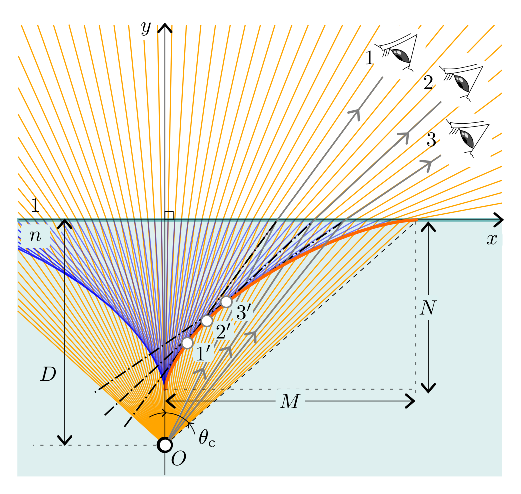
\includegraphics[width=2.7in]{g409.eps}

\section{Derivation of the formula}

Consider a point object O submerged at a depth D below the planar interface 
between air (refractive index $n_1$) and water (refractive index $n_2$). 
A ray of light emanating from O strikes the interface at point A, located a 
distance $\alpha$ from the y-axis. The incident ray makes an angle $\theta_2$ 
with the normal at A, and the refracted ray in air makes an angle $\theta_1$ 
with the same normal.

From Snell's law we have
$$ \sin\theta_1 = \frac{n_2}{n_1} \sin\theta_2 = n\sin\theta_2.$$
The extension of refracted ray is described by the equation 
$$y=k(x-\alpha),$$
where 
$$k=\dfrac{1}{\tan\theta_1}=\dfrac{\cos\theta_1}{\sin\theta_1},$$
and considering the Snell's law,
$$k=\dfrac{\sqrt{1-n^2\sin^2\theta_2}}{n\sin\theta_2}.$$

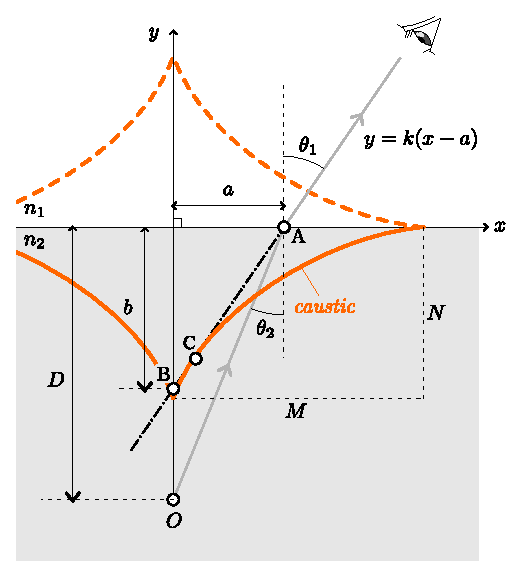
\includegraphics[width=3in]{g237.eps}

This line meets the $y$-axis at B($y=\beta$), thus
$$\beta = -k\alpha.$$

By the geometry we have
$$\alpha = D\tan\theta_2 = \dfrac{D\sin\theta_2}{\cos\theta_2},$$
and
$$\begin{aligned}
	\beta &= -k\alpha \\
	&= -\dfrac{D\sin\theta_2}{\cos\theta_2}
	\dfrac{\sqrt{1-n^2\sin^2\theta_2}}{n\sin\theta_2}\\
	&=-\dfrac{D\sqrt{1-n^2\sin^2\theta_2}}{n\cos\theta_2}.
\end{aligned}$$
Now, let $K=\alpha/M$ and $H=\beta/N$, then
$$ \begin{aligned}
	K^2 + H^2 &= \dfrac{\alpha^2}{M^2}+\dfrac{\beta^2}{N^2}\\
	&=\dfrac{\left(n^2-1\right)\sin^2\theta_2 + 1-n^2\sin^2\theta_2}
	{\cos^2\theta_2}\\
	&=\dfrac{1-\sin^2\theta_2}{\cos^2\theta_2}\\
	&=1
\end{aligned}$$

We introduce dimensionless parameters $\xi=x/M$ and $\eta=y/N$. 
As the POV traverses the $xy$-plane, the corresponding points transform accordingly:
Point $\mathrm{A}(\alpha, 0)$ in object space maps to $\mathrm{K}(K, 0)$ in the $\xi\eta$-plane 
and point $\mathrm{B}(0, \beta)$ in object space maps to $\mathrm{H}(0, H)$ in the $\xi\eta$-plane. 
Crucially, the distance between these transformed points remains constant and equal 
to unity throughout the movement of the POV.

\hfill 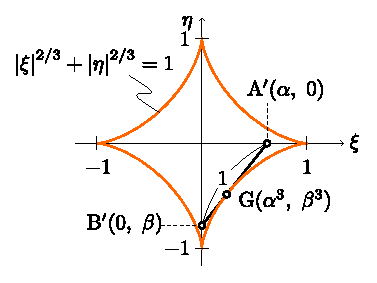
\includegraphics{g107.eps} \hfill\null

The locus of the segment $\overline{\mathrm{KH}}$ in the $\xi\eta$-plane, generates an envelope, which is a 
well-defined geometric shape known as an astroid (not to be confused with an asteroid). 
Mathematically, an astroid is described by the following equation:

$$ \left| \xi \right|^{2/3} + \left| \eta \right|^{2/3} = 1 $$

The image of the submerged object is located at the point of tangency (point $\mathrm{C}$) 
between the segment $\overline{\mathrm{AB}}$(in object space) and the squashed astroid 
envelope in the $xy$-plane. This tangency point signifies the point of divergence for the 
neighboring bundle of light rays. The corresponding coordinates of point $\xi\eta$-plane is 
$\mathrm{G}(K^3, H^3)$.

Thus we can obtain the coordinates of image $(x_{\mathrm{C}}^{}, y_{\mathrm{C}}^{})$ 
from the relation
$$ \left\{ 
\begin{aligned}
	\xi_{\mathrm{C}}^{} &= \dfrac{x_{\mathrm{C}}^{}}{M} = K^3 = \dfrac{\alpha^3}{M^3},\\
	\eta_{\mathrm{C}}^{} &= \dfrac{y_{\mathrm{C}}^{}}{N} = H^3 = \dfrac{\beta^3}{N^3}.
\end{aligned}
\right.$$

That is
$$ \left\{ 
\begin{aligned}
	x_{\mathrm{C}}^{} &= \dfrac{\alpha^3}{M^2},\\
	y_{\mathrm{C}}^{} &= \dfrac{\beta^3}{N^2}=-\dfrac{k^3\alpha^3}{N^2}.
\end{aligned}
\right.$$

Using 
$$\sin\theta_2 = \dfrac{\alpha}{\sqrt{D^2+\alpha^2}},$$
we have
$$k = \dfrac{\sqrt{D^2-(n^2-1)\alpha^2}}{n\alpha},$$
and we can derive the position of the image as parametric functions w.r.t. $\alpha$:
$$ \left\{ 
\begin{aligned}
	x_{\mathrm{C}}^{} &= (n^2-1)\dfrac{\alpha^3}{D^2},\\
	y_{\mathrm{C}}^{} &= -\dfrac{n^2}{D^2}\dfrac{\alpha^3}{n^3\alpha^3}\left\{ D^2-(n^2-1)\alpha^2 \right\}^{3/2}\\
	&=-\dfrac{D}{n}\left\{ 1-(n^2-1)\dfrac{\alpha^2}{D^2} \right\}^{3/2}.
\end{aligned}
\right.$$

\section{POV under water}
When an object is located at a height $D$ above a planar interface separating 
air and water, and the point of observation (POV) is submerged in water, the 
relative refractive index is less than unity, i.e., $1/n < 1$. Through similar 
reasoning, the equation for the caustic can be derived as:

$$ \left| \xi \right|^{2/3} - \left| \eta \right|^{2/3} = -1, $$

where $\xi = \dfrac{x}{W} $, $\eta = \dfrac{y}{Z}$, 
$W = \dfrac{nD}{\sqrt{n^2-1}}$, and $Z = nD$. This curve exhibits asymptotes 
with slopes of $\pm Z/W = \pm \sqrt{n^2-1}$. 

Consequently, the observed imagery of the \emph{skyscape} above the water, 
as viewed from underwater, is compressed into a circular region (or more 
accurately, a cone) bounded by the critical angle of total internal reflection, 
commonly referred to as Snell's window. This circular, wide-angle view, as 
perceived by an underwater observer, bears a resemblance to the field of view 
captured by a fisheye lens.

To the best of the author's knowledge, a specific name for this shape of the 
caustic curve has not been established in the literature. Given that the 
generalized form of this curve, 

$$ \left| \xi \right|^{2/3} - \left| \eta \right|^{2/3} = \pm1, $$
has physical significance as the caustic of rays emanating from a point light 
source above water and refracted into water, and given its relationship to 
the astroid, analogous to the relationship between a hyperbola and an ellipse, 
the term \emph{hyperastroid} is proposed as a suitable nomenclature.\\

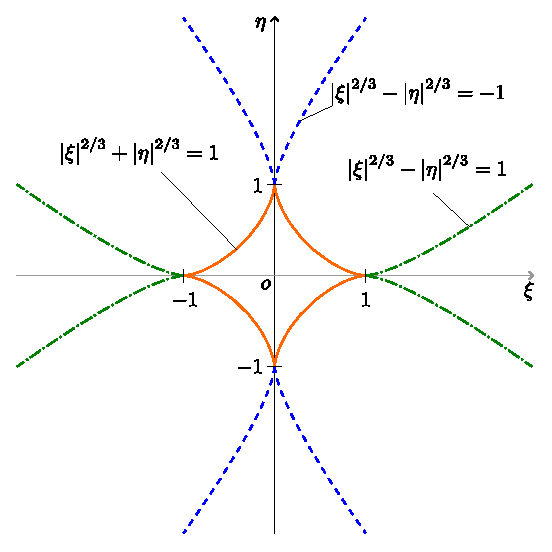
\includegraphics[width=3in]{g254.eps}

The astroid is a member of the 
family of curves named \href{https://mathworld.wolfram.com/Astroid.html}{\emph{superellipse}}, which is defined by 
$$ \left| \xi \right|^{r} + \left| \eta \right|^{r} = 1. $$

Asteroid is the case where $r=2/3$. But as far as I know nor is there a name for the 
family of curves in the form
$$ \left| \xi \right|^{r} - \left| \eta \right|^{r} = \pm 1, $$
which could be named \emph{super-hyperbola}, although the repeating cognates may 
bother you\footnote{I might suggest \emph{superbola}.}.

\section{Finding the Image Location}
Since we can obtain a closed form of the caustic, we can find the location of the 
image given the object and the POV as follows.

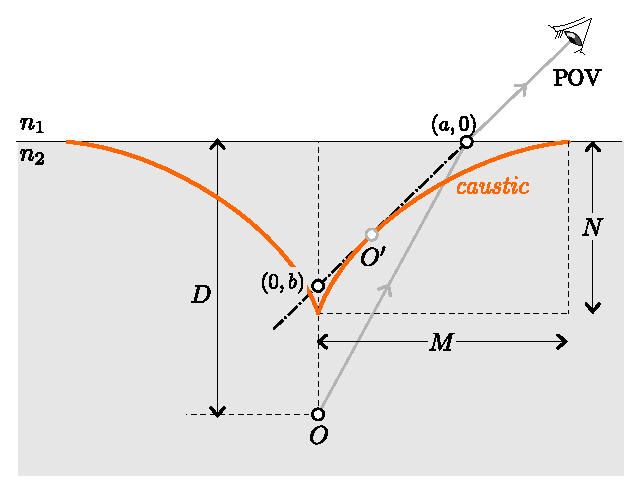
\includegraphics[width=3in]{g394.eps}

A tangent line is drawn from the POV to the caustic curve. The point of tangency 
between the tangent line and the caustic represents the location of the image of 
the point source. Simultaneously, the intersection point of this tangent line 
with the water surface identifies the point of incidence of the light ray 
originating from the object.

For an extended object within the water, the image of each point on the object's 
surface can be determined by applying the same procedure. The locus of these 
individual image points, as the point moves continuously along the object's 
surface, constitutes the image of the extended object.

\includegraphics*[width=3in]{g240.eps}

However, it is difficult, if not impossible, to find the tangent line to the caustic analytically, and 
in practice, we must be satisfied with finding an approximate value using numerical 
methods.

Another method is to numerically find the path of the light ray connecting the object 
and the viewpoint using Fermat's principle, and then find the location of the image 
by using the tangent point formula of the astroid based on the coordinates of the 
point where the light ray intersects the water surface. A Python example for this can 
be found at \href{https://github.com/mingshey/python_projects/blob/main/Refraction_Image_en.ipynb}%
{github.com/mingshey/python\_projects}.

\appendix
\newcommand{\pardiff}[2]{{\frac{\partial #1}{\partial #2}}}
\newcommand{\ilpardiff}[2]{{{\partial #1}/{\partial #2}}}
\section*{Note: Astroid as an envelope}
Let's assume that a point $(K, 0)$ on the x-axis and a point $(0, H)$ on the y-axis in a Cartesian plane move while maintaining a constant distance $a$ between them. Then, $K^2+H^2=a^2$, and the equation of the line containing the line segment at a certain moment can be written as
$$y=-\dfrac{H}{K}(x-K)$$
and using $H=\pm \sqrt{a^2-K^2}$, we have
$$y(x, K) = \mp \dfrac{\sqrt{a^2-K^2}}{K}(x-K)$$
As the value of $K$ changes, the line segment or line connecting the two points changes, and the envelope drawn by it is the locus of stationary points at each moment, that is, the locus of points where $\ilpardiff{y}{K} = 0$. Let's find the $(x, y)$ that satisfy this condition.

$$ \begin{aligned}
	\pardiff{y}{K} &= \pm\left[\left( \dfrac{1}{\sqrt{a^2-K^2}}+\dfrac{\sqrt{a^2-K^2}}{K^2}\right) (x-K) + \dfrac{\sqrt{a^2-K^2}}{K} \right]\\
	&= \pm \dfrac{(K^2+a^2-K^2)(x-K)+K(a^2-K^2)}{K^2\sqrt{a^2-K^2}}\\
	&= \pm \dfrac{a^2 x - K^3}{K^2 \sqrt{a^2 - K^2}}\\
	&= 0.
\end{aligned}
$$
Therefore the abscissa of the stationary point is $x = K^3/a^2$, and its ordinate is

$$ \begin{aligned}
	y(x, K) &= \mp \dfrac{\sqrt{a^2-K^2}}{K}\left(\dfrac{K^3}{a^2}-K\right)\\
	& = \pm \dfrac{\left( a^2- K^2 \right)^{3/2}}{a^2}\\
	& = \dfrac{H^3}{a^2}
\end{aligned}
$$
Therefore, the coordinate $(x, y)$ of the stationary points satisfies the equation
$$ \left|\dfrac{x}{a}\right|^{2/3} + \left|\dfrac{y}{a}\right|^{2/3} = 1. $$
$\blacksquare$

\end{document}

